\section{Background} \label{sect:backgroundw}

In this project, we will study the performance benefits of running algorithms on the GPU in parallel. To do this we will implement three linear algebra algorithms in increasing degrees of complexity, namely: Matrix addition, matrix multiplication, and QR-decomposition.

% Lav et intro afsnit der bedre introducerer meningen med opgaven.

First, we will implement these on the CPU to establish a baseline implementation. Next, we will implement them on the GPU, and hopefully see a performance increase.

This section will outline the mathematical formulas we will implement as algorithms, and the basics of CPU and GPU architecture.

\subsection{Linear Algebra}

\subsubsection{Matrix addition}

The first algorithm we want to implement is the matrix addition formula. Assume two \(m \cdot n\) matrices \(\mathbf{A}\) and \(\mathbf{B}\). 

\[\mathbf{C} = \mathbf{A} + \mathbf{B}\]

Computing the sum of the matrices is done by adding each element \(i,j\) pairwise, where \(i\) and \(j\) are indices for the elements of the matrices.

\[c_{ij} = a_{ij} + b_{ij}\]

\begin{figure}[H]
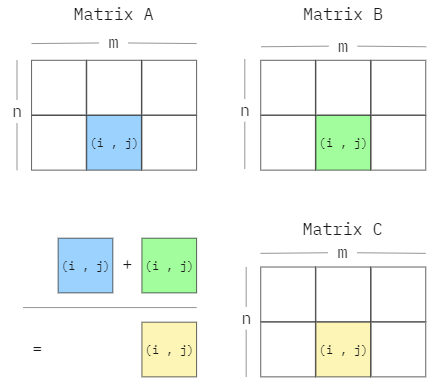
\includegraphics[scale=.65]{Documents/Report/Figures/MatrixAddition.png}
\centering
\caption{Single element addition calculation.}
\label{fig:addition_illustration}
\end{figure}

\subsubsection{Matrix multiplication}

Next we want to implement matrix multiplication. Matrix multiplication \(\mathbf{A} \cdot \mathbf{B}\) requires matrix \(\mathbf{A}\) to have dimensions \(l \cdot m\) and matrix \(\mathbf{B}\) to have dimensions \(m \cdot n\). This means that the column count of matrix \(\mathbf{A}\) must be equal to the row count of matrix \(\mathbf{B}\).

\[\mathbf{C} = \mathbf{A} \cdot \mathbf{B}\]

In matrix multiplication, element \(c_{i,j}\) is calculated from the $i^{th}$ row of matrix \(\mathbf{A}\), call it \(a_{i \cdot}\) and the $j^{th}$ column of matrix \(\mathbf{B}\), call it \(b_{\cdot j}\). Both \(a_{i \cdot}\) and \(b_{\cdot j}\) have $m$ many elements. To calculate element \(c_{i,j}\), multiply each element \(a_{ik}\) with \(b_{kj}\), where $1 \leq k \leq m$. Then calculate the sum of these products.

\[c_{i,j} = \sum_{k=1}^m a_{ik} b_{kj}\]

\begin{figure}[H]
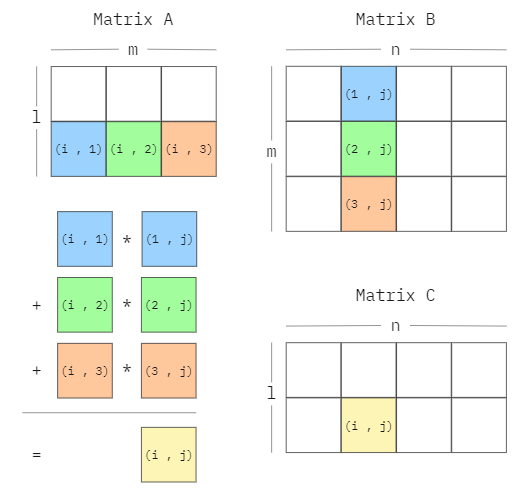
\includegraphics[scale=.65]{Documents/Report/Figures/MatrixMultiplication.png}
\centering
\caption{Single element multiplication calculation.}
\label{fig:multiplication_illustration}
\end{figure}

An appealing way to understand matrix multiplication is to interpret it geometrically. Assume a vector space where the basis vectors can be represented as a matrix $\mathbf{A}$. To multiply this matrix with another matrix $\mathbf{B}$ can be interpreted such that the basis vectors are linearly transformed to new positions. For example, all vectors might be stretched by a factor of 2 and rotated clockwise by 10 degrees. 

\subsubsection{QR-decomposition}
The final algebraic algorithm we want to implement is QR-decomposition. This algorithm takes in a matrix \(\mathbf{A}\) and factorizes it into matrices \(\mathbf{Q}\) and \(\mathbf{R}\).

\[\mathbf{A} = \mathbf{Q} \cdot \mathbf{R}\]

\noindent Here, \(\mathbf{Q}\) is an orthogonal matrix such that 

\[\mathbf{Q^T \cdot Q = I}\]

where \(\mathbf{Q^T}\) is the transpose of \(\mathbf{Q}\) and \(\mathbf{I}\) is the identity matrix. This property also means that \(\mathbf{Q}\) is symmetrical along the diagonal. \(\mathbf{R}\) is an upper triangular matrix, where all elements below the diagonal are 0. 

% Explain why this is useful. I.e. linear algebraic equations and how to solve them with this.

The Householder matrices \(\mathbf{Q_i}\) for \(\mathbf{Q_1 \ldots Q_{n}}\) are computed for each column in our matrix \(\mathbf{A}\). This leaves us with a way to calculate \(\mathbf{Q}\) if we need it.\cite[Sect. 2.13, 11.2]{numericalrecipes}

\[\mathbf{Q = Q_1 \cdot Q_1 \cdot \ldots \cdot Q_{n}}\]

% Talk more in-depth aboout Householder (why it is hard to parallelize it).
% Mention Givens and that it is less numerically stable, but easier to parallelize.

Geometrically, \(\mathbf{Q}\) can be interpreted as a linear transformation that rotates and reflects the basis vectors. Likewise, \(\mathbf{R}\) can be interpreted as a linear transformation that scales and shears the basis vectors. Therefore, by computing the QR-decomposition, we factorize a matrix into these two kinds of linear transformations. 

% What else we can include in this section on what the algorithm does

% we dont understand some of the math
% implementation from the book
% our iteration on the algorithm (TDD)
% running the loop one more time
% an iterative algorithm, the computes columns in sequence
% numerical stbility (dividing by scale)
% calculating the inner product


\newpage
\subsection{CPU and GPU Architecture}

\subsubsection{The CPU}

The part of the computer called the \textit{Central Processing Unit} (CPU) is typically responsible for executing code. When executing code, the CPU is performing instructions on some data. Those instructions and data often reside in \textit{main memory}. Main memory uses \textit{Dynamic Random Access Memory} (DRAM), which is about 10x slower than \textit{Static Random Access Memory} (SRAM) \cite[p. 561-562]{computersystems}. The CPU has much less SRAM than DRAM is available, due to SRAM being more expensive in terms of production costs and electricity.

A simplified overview of the CPU's architecture and its relation to main memory can be seen in figure \ref{fig:cpu_architecture}. It can be seen that the main memory is located in a physically different place than the CPU, connected by memory busses and an I/O bridge. The CPU also has a very limited on-chip storage called the \textit{cache memories}, that use SRAM.

If the CPU had to get data from main memory every time it read some data, it would slow down the computer a lot. Therefore, when the CPU reads from main memory, it also reads nearby data and writes it to its cache in anticipation that it might need it soon. When a computer program takes advantage of this, it is said to have good \textit{spatial locality} \cite[p. 640]{computersystems}.

\begin{figure}[h]
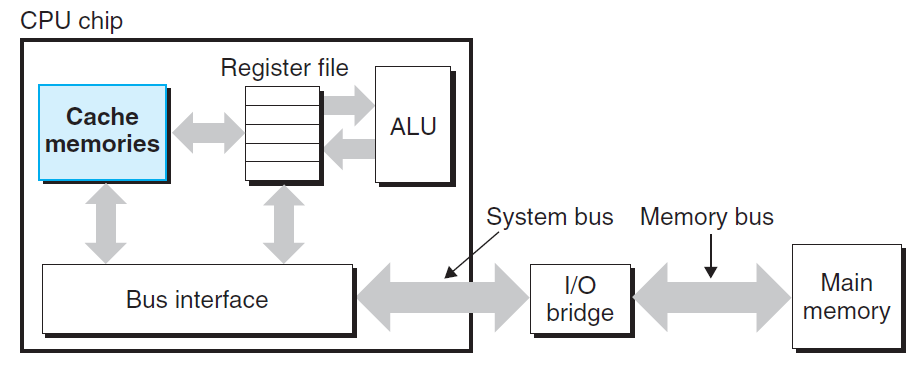
\includegraphics[width=\textwidth]{Documents/Report/Figures/CPU Architecture.png}
\caption{Overview of CPU Architecture. From \cite{computersystems}}
\label{fig:cpu_architecture}
\end{figure}

The CPU also has a \textit{register file}, where there is a number of word-sized\footnote{Depending on the specific CPU, word-size may vary, but usually, a word is either 32-bits or 64-bits.} registers, each with a distinct name, where the CPU can store anything that fits in a word. This register file is \textit{very} limited in terms of size, but it is accessible to the CPU in 0 cpu cycles.\cite[p. 9-10]{computersystems}. It is therefore at least 10x faster than the cache, and at least 100x times faster than the main memory.

The CPU has an \textit{Arithmetic and Logic Unit} (ALU) that it uses for arithmetic operations (i.e. additions, multiplications) and logical operations (i.e. comparisons).

The CPU has a set of instructions (called the instruction set) that appear very simple on the surface. An instruction may say "move the value of register 8 into register 9" or "add the values from to registers together". In reality however, most modern CPUs have much more sophisticated mechanisms to enable better performance, such as branch prediction and instruction-level parallelism. These low-level details are often called the CPU's \textit{microarchitechture} \cite[p. 10]{computersystems}.\\

\noindent For many years CPU cores got faster and faster. However, this development plateaued in the early 2000s. Instead, more cores were fit into the CPUs and multi-core processors became the norm \cite{karlrupp:processor_trend_data}.

On modern computers a CPU will contain anywhere from 2 to 90+ cores, typically in the 4-12 core range with consumer CPUs. Each core can efficiently execute a series of instructions sequentially, and each core has its own cache, as well as a shared cache between the cores.

Therefore, to run programs efficiently on a modern CPU, one should utilize all its cores by writing code which can run in parallel. This is usually done with the abstraction of \textit{threads}, which are fundamentally a sequence of instructions \cite[p. 1022]{computersystems}.

\subsubsection{The GPU} \label{background_gpu}

\noindent Another component in the computer capable of executing code is called the \textit{Graphics Processing Unit} (GPU). Likewise, it has a set of cores capable of executing instructions. However, the GPU was built to process massive amounts of data in parallel. Thus, the architectural structure of the GPU is different from the CPU.

The GPU is often referred to as \textit{many-core} rather than \textit{multi-core}. Instead of having a single- or double-digit amount of cores, consumer-level GPUs, usually have a three-, four- or even five-digit amount of cores, enabling many more instructions to be executed in parallel. This increase in cores comes at the cost simpler GPU cores, compared to GPU cores, as seen in \ref{fig:cpu_vs_gpu} \cite[Sect. 1.1]{nvidia:cudadoc}. A GPU core does not have all the microarchitecture that a CPU core has, and is therefore slower. An arbitrary program running single-core on a modern CPU would be faster than the same program running single-core on a GPU.

\begin{figure}[ht]
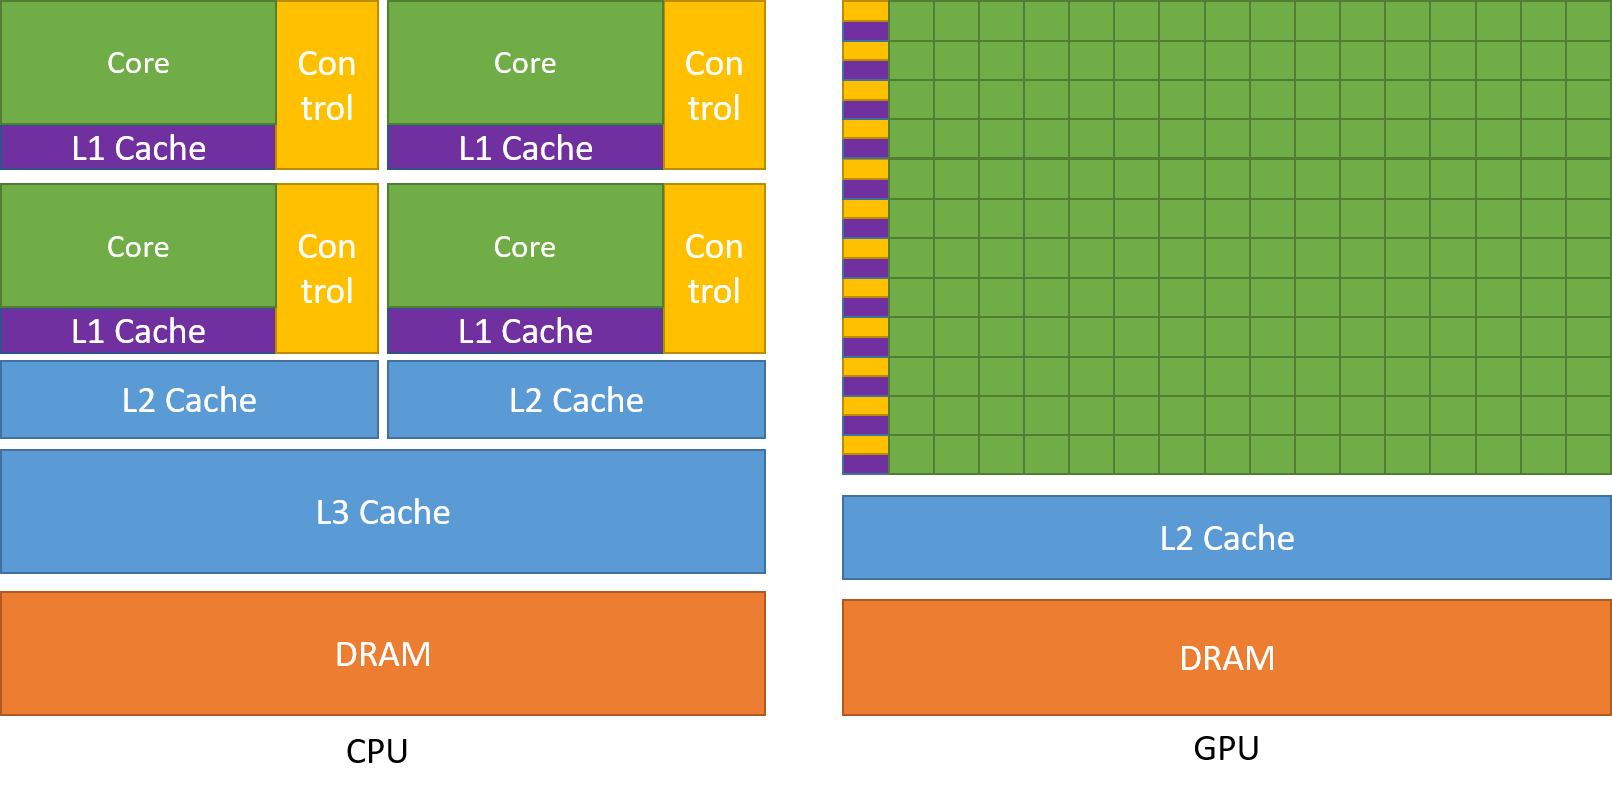
\includegraphics[width=\textwidth]{Documents/Report/Figures/CPU vs GPU .png}
\caption{Overview of CPU Architecture and GPU Architecture. From \cite{nvidia:cudadoc}}
\label{fig:cpu_vs_gpu}
\end{figure}

The GPU also do not have a cache for each core. Instead they have a \textit{level 1} (L1) cache for each \textit{Streaming Multiprocessor} (more on that later). They also have a \textit{level 2} (L2) cache that is shared between all cores on the GPU. On the GPU, memory is referred to as \textit{Video Random Access Memory} (VRAM).

So, the appeal for a GPU is not the performance and capabilities of each individual core, but rather the \textit{amount} of cores it has.

\noindent The GPU manufacturer NVIDIA have created a parallel programming platform called CUDA. CUDA can be used in handful of languages, but for this project we use the CUDA C/C++ language extensions. These introduce some key abstractions, namely \textit{kernels, threads, thread blocks} and \textit{grids}. 

A kernel represents instructions to be executed $N$ times in parallel, where $N$ is the number of threads to execute the code [Sect. 2.1]\cite{nvidia:cudadoc}. A thread executes a kernel and resides in a thread block, holding multiple threads. A thread block then resides in a grid of blocks as seen in figure \ref{fig:threads and blocks}.

\begin{figure}[ht]
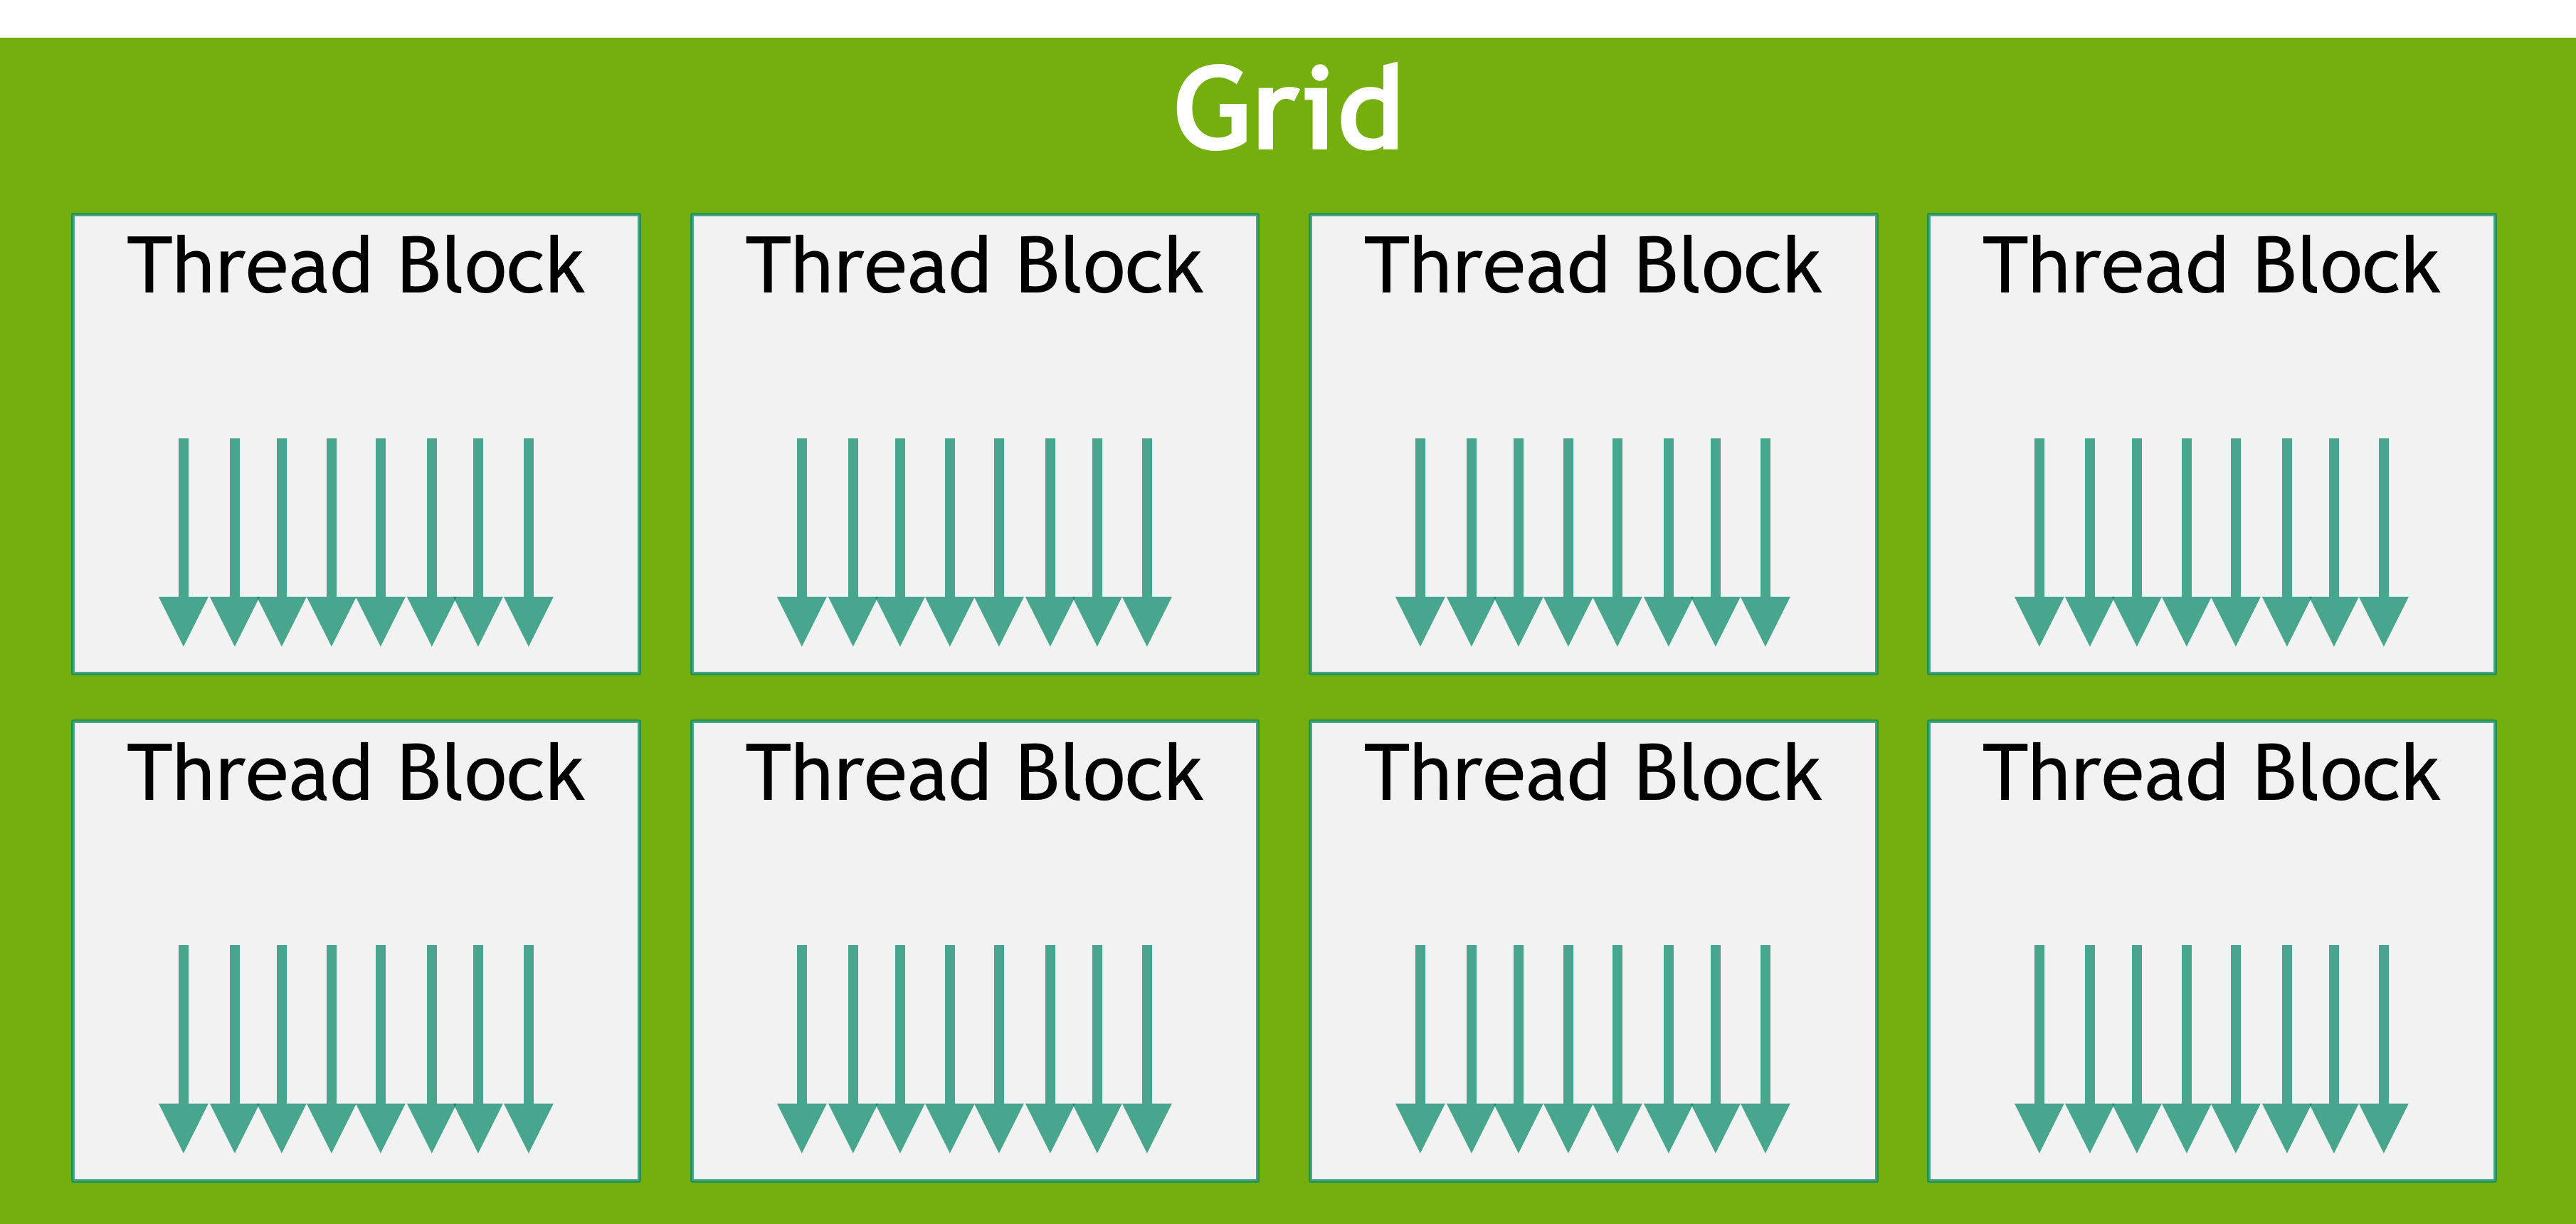
\includegraphics[width=\textwidth]{Documents/Report/Figures/Threads and blocks.png}
\caption{Threads inside thread blocks inside the grid. From \cite{nvidia:cudadoc}}
\label{fig:threads and blocks}
\end{figure}

Thread blocks and grids can be 1-, 2- or 3-dimensional. This is implemented for convenience when working with a 2-dimensional domain like matrices. A thread block can hold up to 1024 threads. The limit is there because all threads of a block are expected to be on the same \textit{streaming multiprocessor core} (SM) [Sect. 2.2]\cite{nvidia:cudadoc}. The GPU consists of an array of streaming multiprocessors. Each have their own memory and control circuit, which allows threads within the same thread block to share a part of the cache, as well as synchronize with each other. 

More powerful GPUs generally have more streaming multiprocessors than less powerful GPUs. The thread block abstraction allows programmers to write efficient code for many types of GPUs, without having to worry about how many SMs they have. A GPU with more SMs will be faster, since they can execute more blocks in parallel, but both a GPU with 2 and 4 SMs will execute in parallel as fast as they are able to. This is illustrated in figure \ref{fig:automatic scalability} in appendix B \cite[Sect. 1.3]{nvidia:cudadoc}.\\

\noindent A typical CUDA program is started by the CPU. In this context, the CPU is called the \textit{host}. The host will likely allocate some GPU memory and copy data over to the GPU. In this context, the GPU is referred to as the \textit{device}. The host will then \textit{launch} the device kernel with special syntax: \texttt{<<<example\_kernel>>>}. When the device kernel has run, the host may then copy over some data from the device to the host and deallocate the memory on the device. So in a CUDA program, both the CPU and GPU has a role to play. 

One could say that the CPU is the manager that organizes everything, while the GPU is the hard working employee.

The typical performance bottleneck in a CUDA program is the communication between the CPU and GPU. Optimizing communication, as well as the parallelization on the GPU, are the keys to optimizing performance of CUDA programs. Specifically, the transfer of data from the host memory to device memory is quite slow \cite[Sect. 5.3.1]{nvidia:cudadoc}.\\

% We could talk about managed memory here?

\noindent We will implement the algorithms to run sequentially on the CPU and in parallel on the GPU. One might argue that a more fair comparison would be to write a parallel program on the CPU and then comparing the performance with the parallel program on the GPU.\footnote{One could also take advantage of SIMD operations on the CPU.}

If the purpose of the project was to judge whether an algorithm should be implemented on the CPU or GPU to yield the best performance, one would be correct. However, the purpose of this project is to implement algorithms on the GPU, and tuning that code to better performance. Writing a GPU implementation faster than a parallel implementation on the CPU is out of scope for this project.

% Afsnit om vores hypoteser. Hvorfor vi skriver denne rapport. 
% Altså at addition ikke vil få en speedup, og hvorfor vi tror det
% at multiplication vil få en speedup, og hvorfor vi tror det